\chapter{Конструкторская часть}
В данном разделе будут приведены схемы алгоритмов, а также оценены трудоемкости каждого из алгоритмов.

\section{Представление алгоритмов}

На вход алгоритмов подается матрица стоимостей $G$ размера $N \times N$; на выходе - минимальная стоимость маршрута $minCost$, а также сам маршрут, представленный последовательностью посещенных городов $bestRoute$.

Для муравьиного алгоритма на вход также требуются следующие параметры: коэффициент влияния феромона $alpha$, коэффициент испарения феромона $rho$, максимальное количество итераций $tmax$, количество обычных муравьев $numA$, количество элитных муравьев $numEA$.

На рисунках~\ref{fig:classic} ---~\ref{fig:season} приведены схемы двух алгоритмов, используемых в методах решения задачи коммивояжера: полного перебора, муравьиного.

\clearpage

\begin{figure}[h]
	\centering
	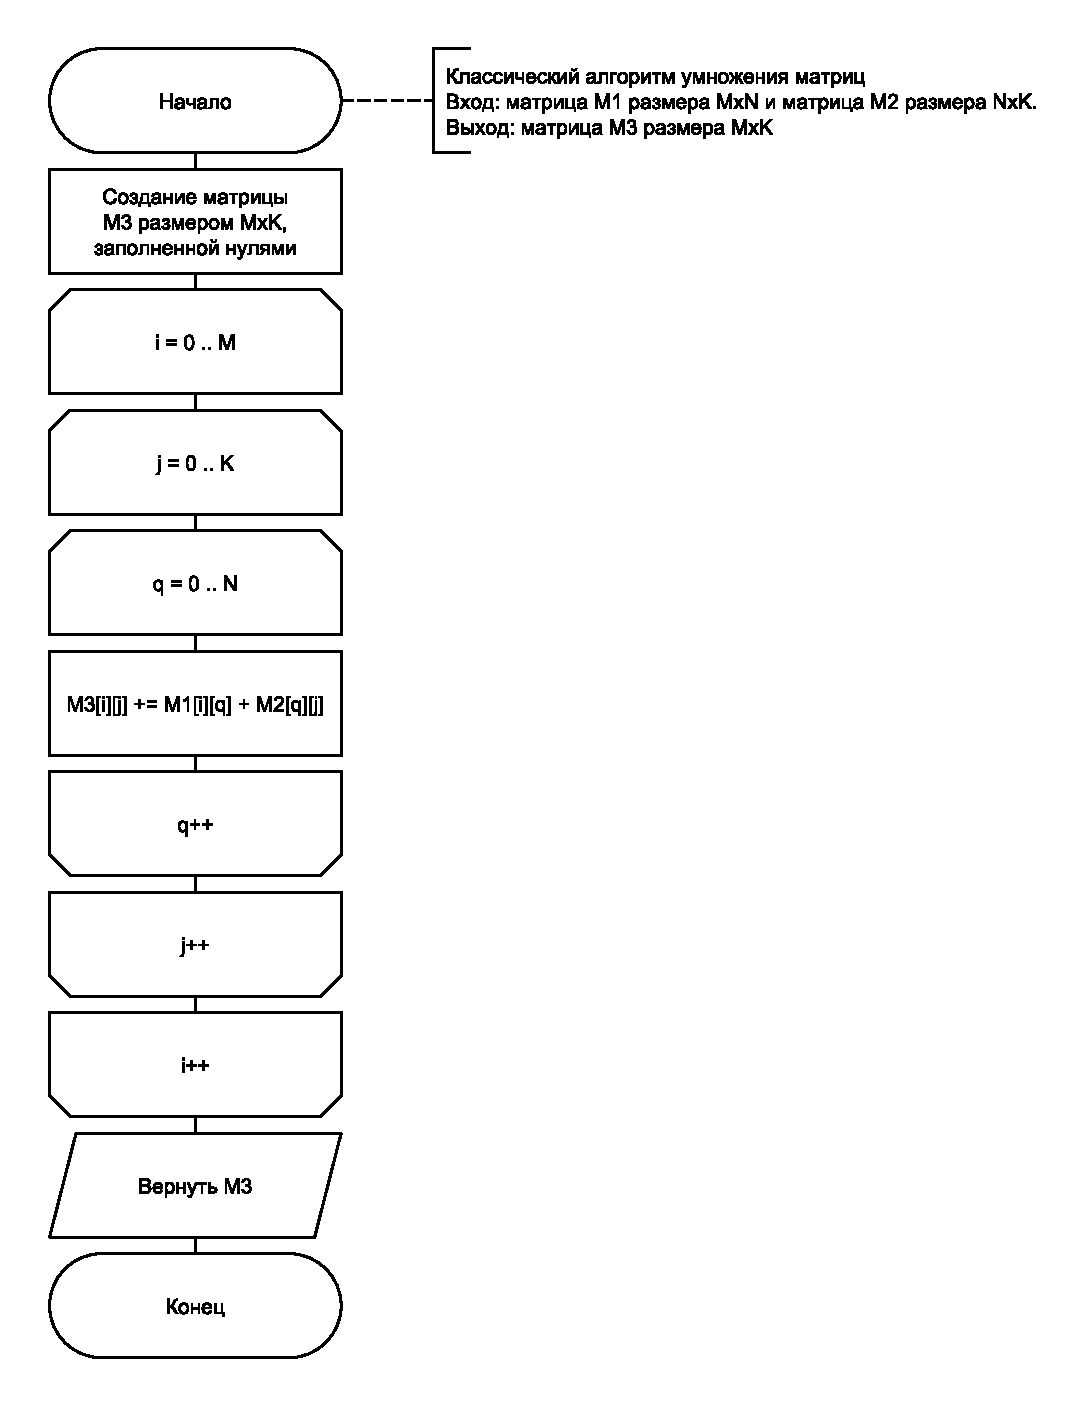
\includegraphics[scale=0.7]{img/classic.eps}
	\caption{Схема алгоритма полного перебора}
	\label{fig:classic}
\end{figure}

\clearpage

\begin{figure}[h]
	\centering
	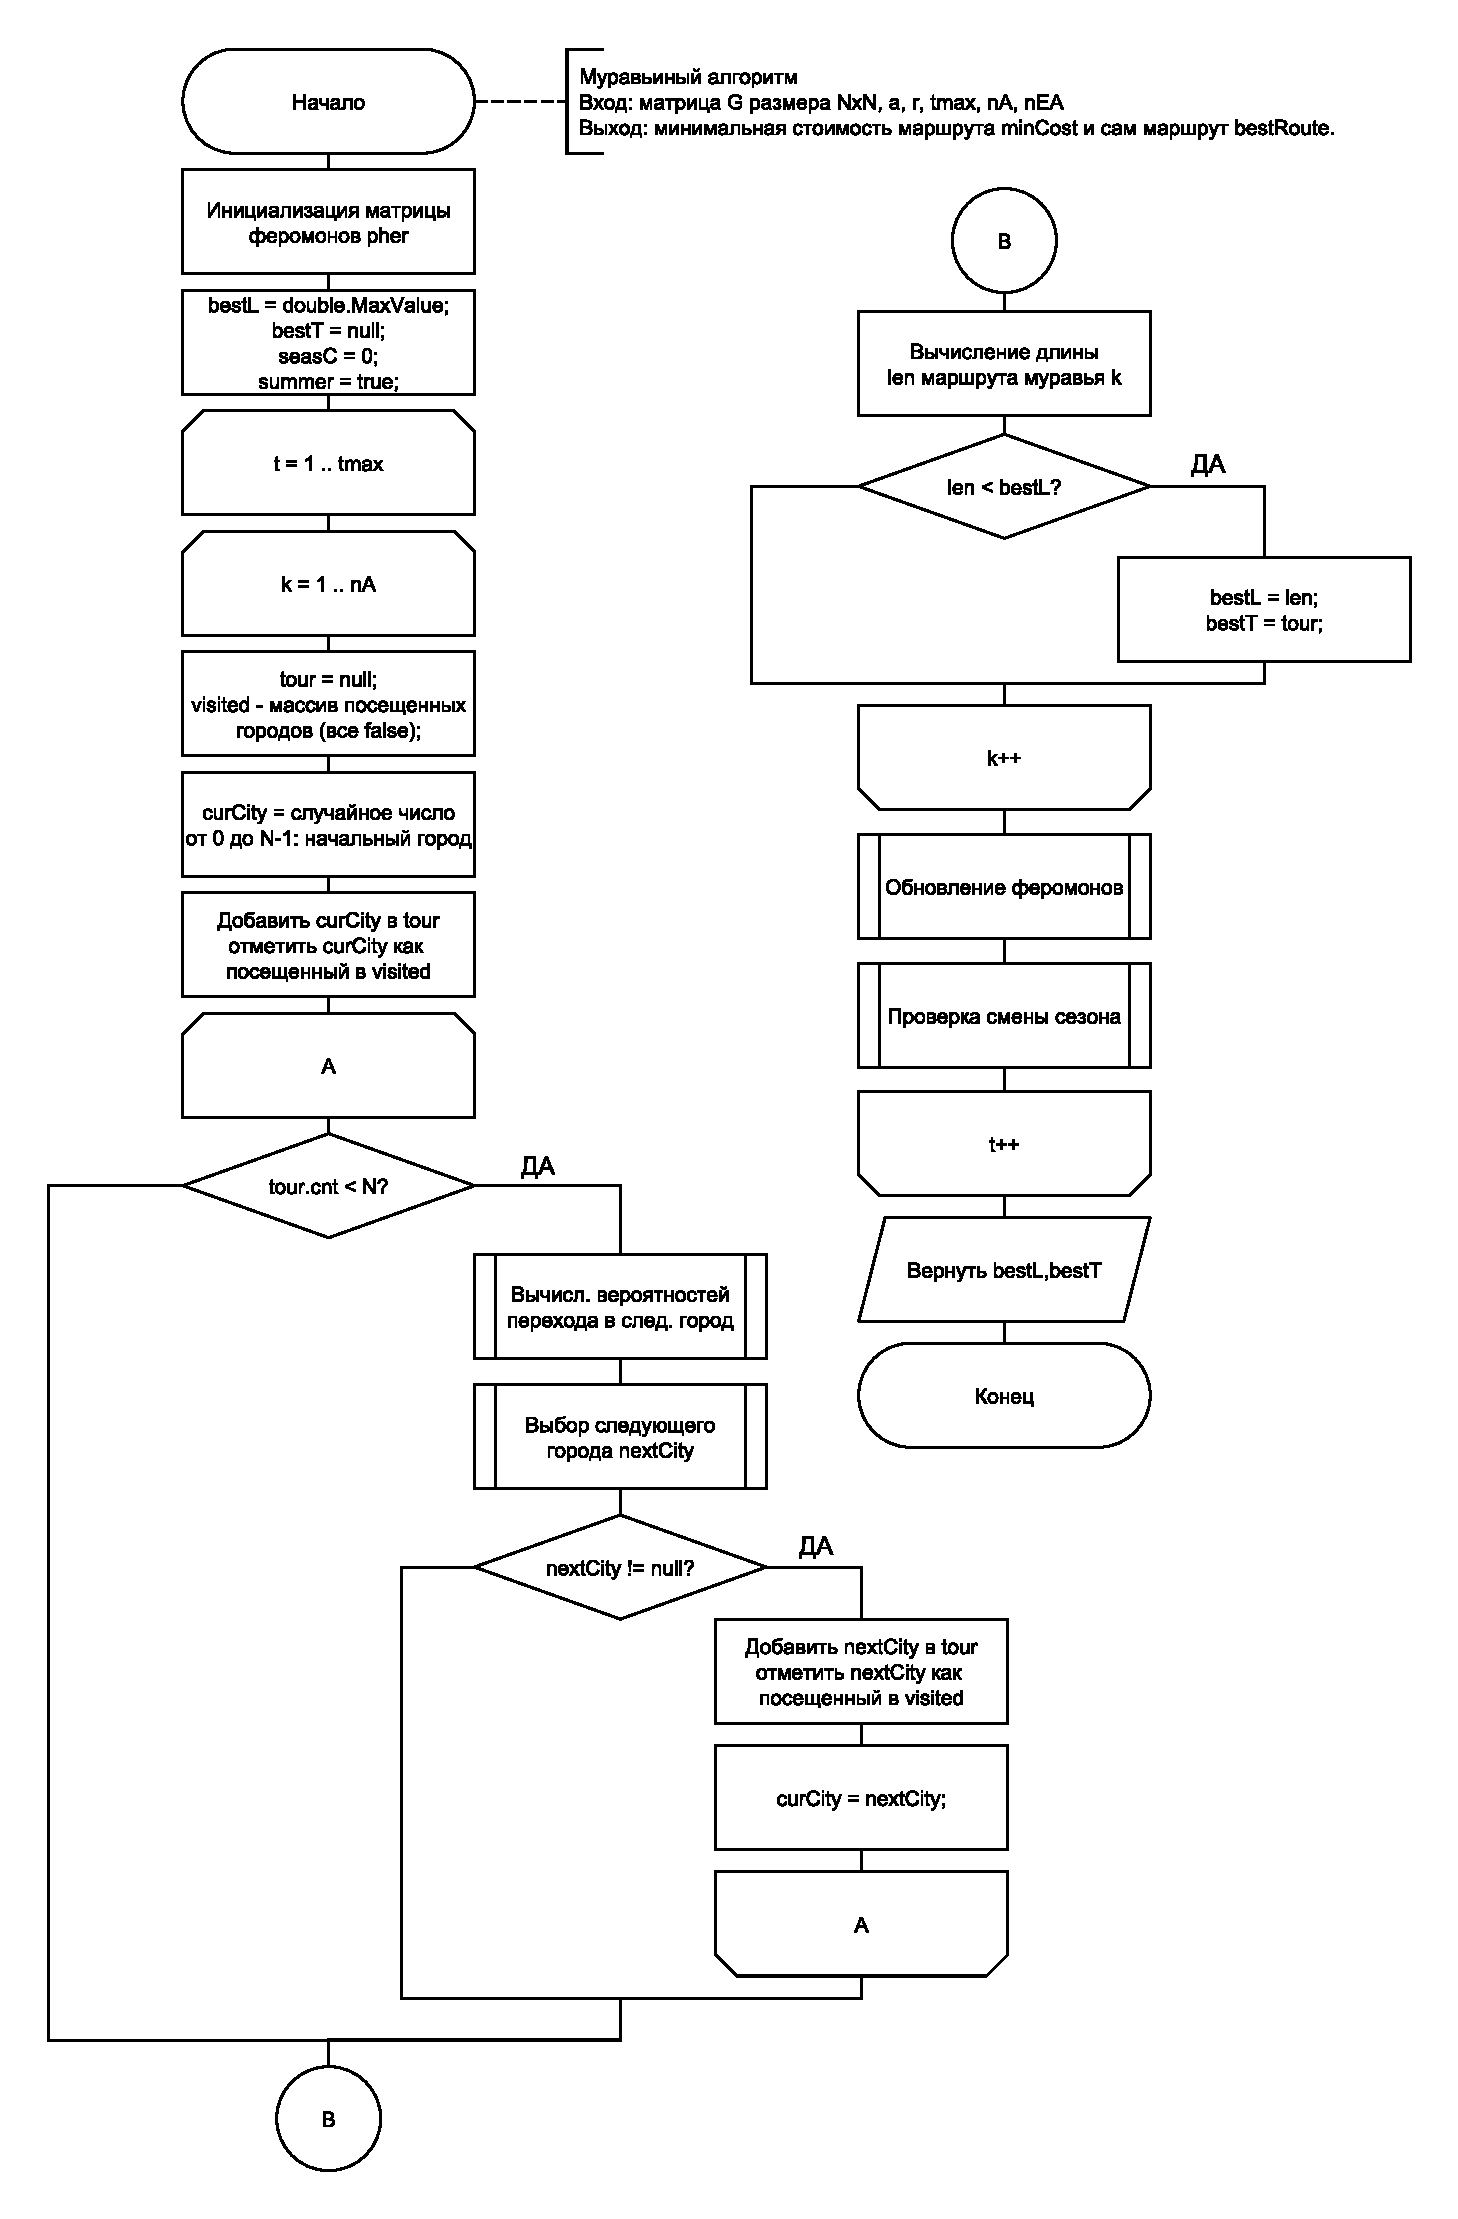
\includegraphics[scale=0.65]{img/antlgo.eps}
    \caption{Схема муравьиного алгоритма}
	\label{fig:antlgo}
\end{figure}
\begin{figure}[h]
	\centering
    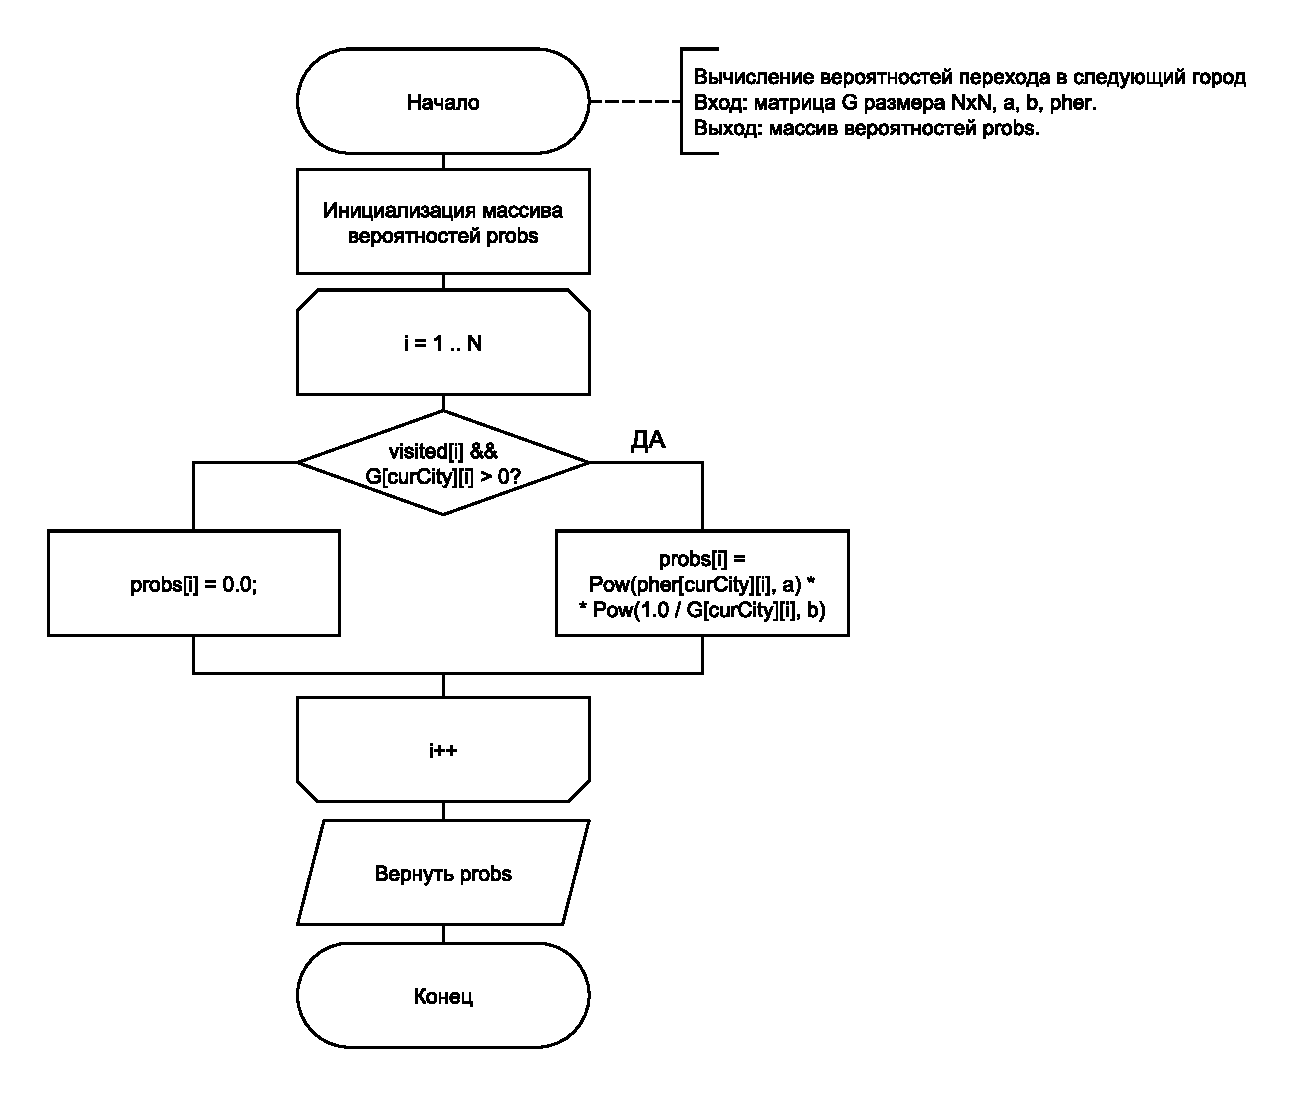
\includegraphics[scale=0.6]{img/probcalc.eps}
	\caption{Схема вычисления вероятностей}
	\label{fig:vinograd}
\end{figure}
\begin{figure}[h]
	\centering
    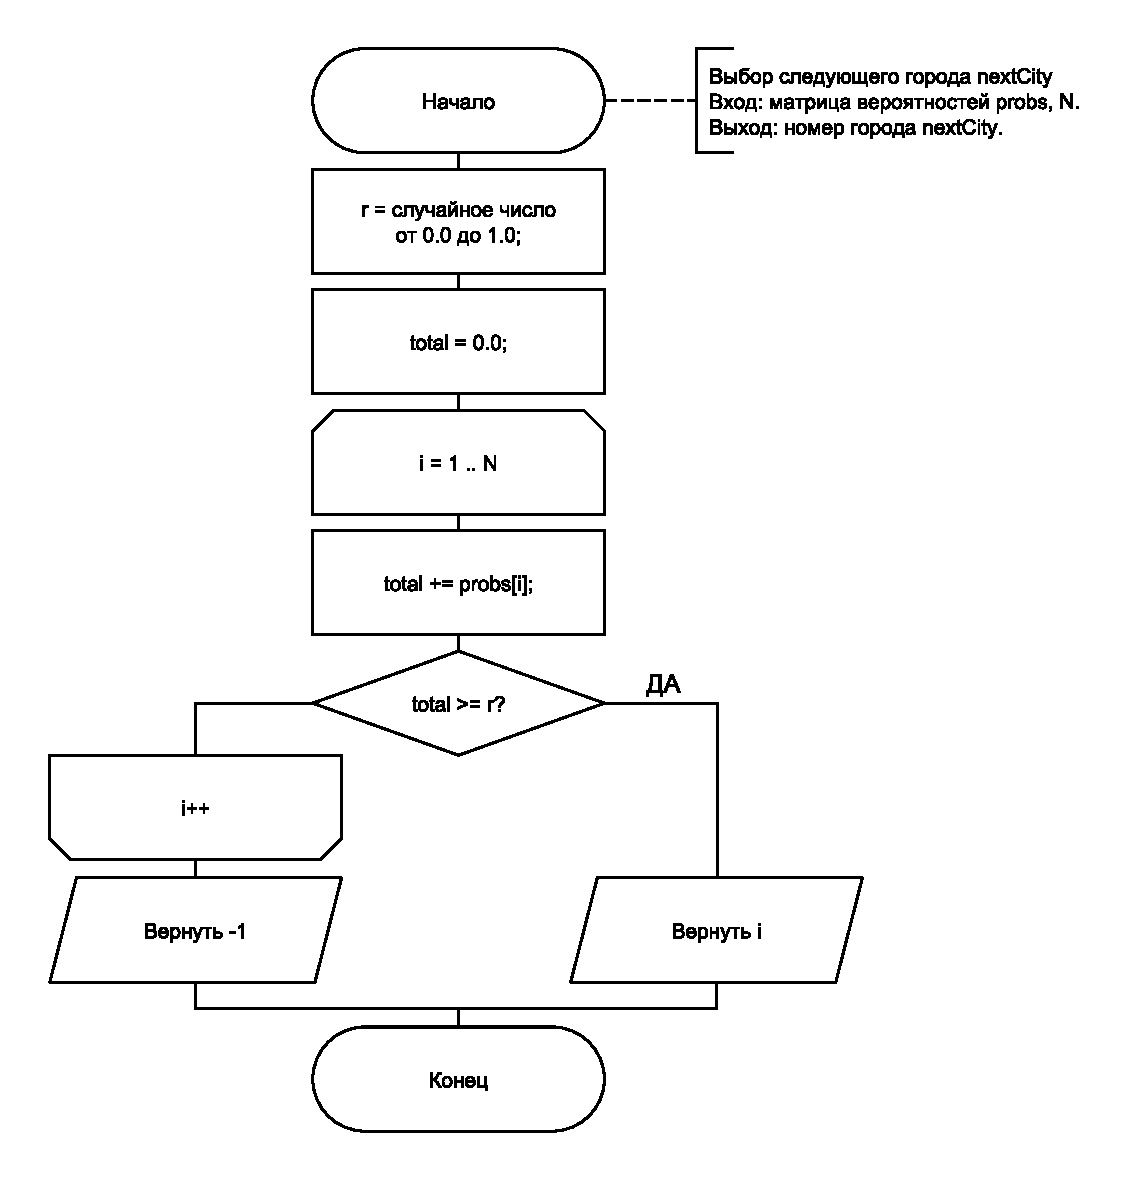
\includegraphics[scale=0.6]{img/citycalc.eps}
	\caption{Схема вычисления нового города}
	\label{fig:vinograd}
\end{figure}
\begin{figure}[h]
	\centering
    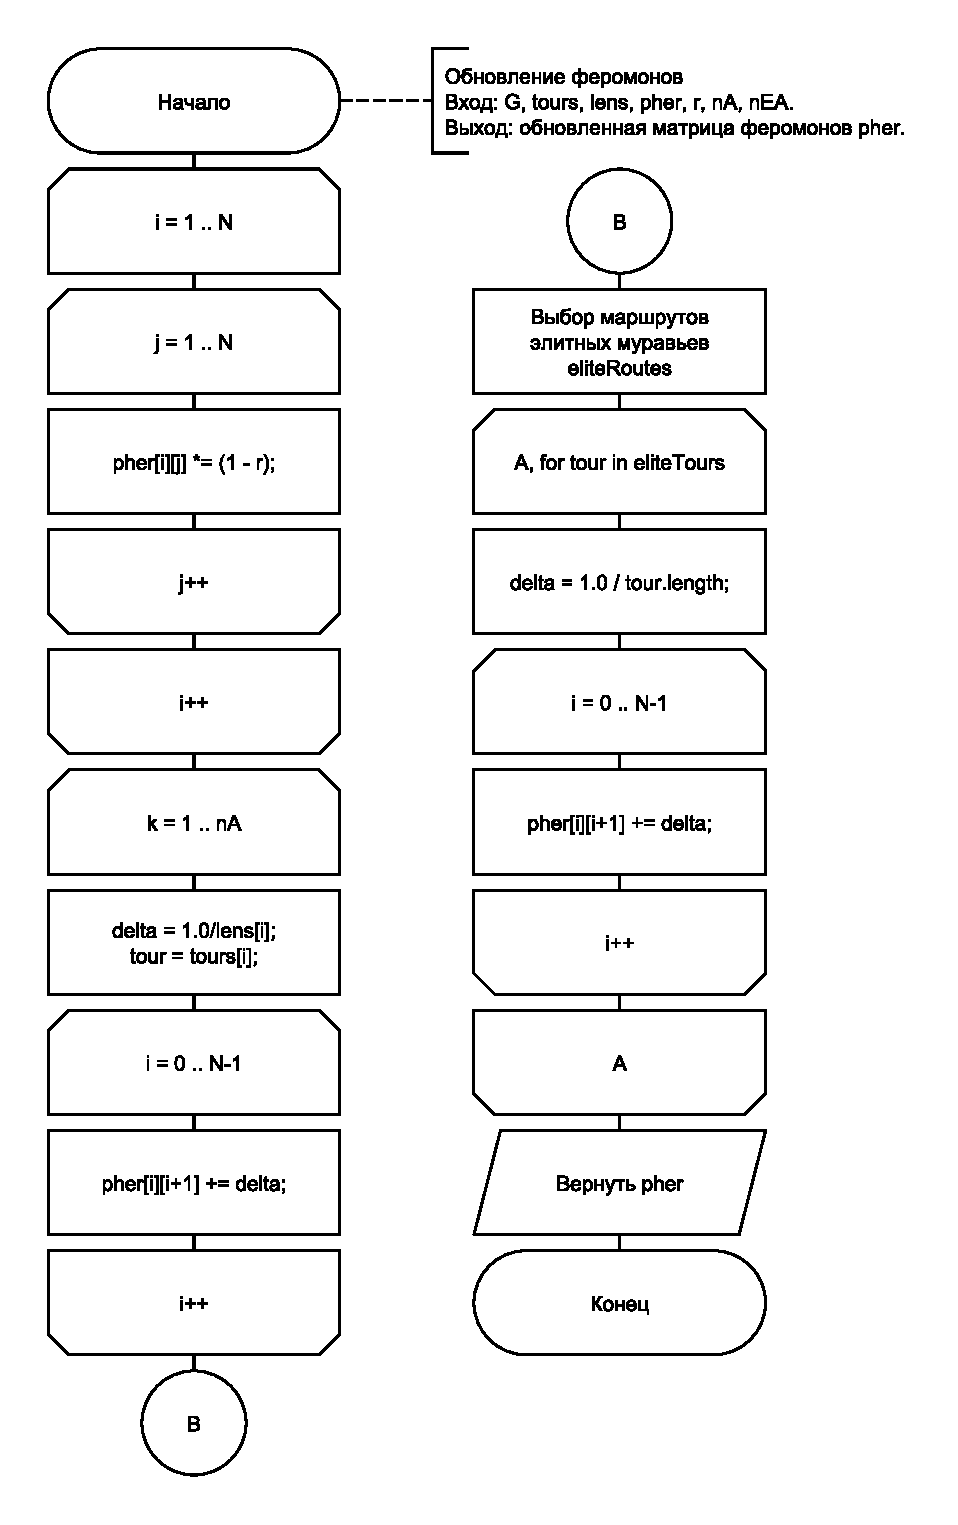
\includegraphics[scale=0.75]{img/pherupd.eps}
	\caption{Схема обновления феромонов}
	\label{fig:vinograd}
\end{figure}
\begin{figure}[h]
	\centering
	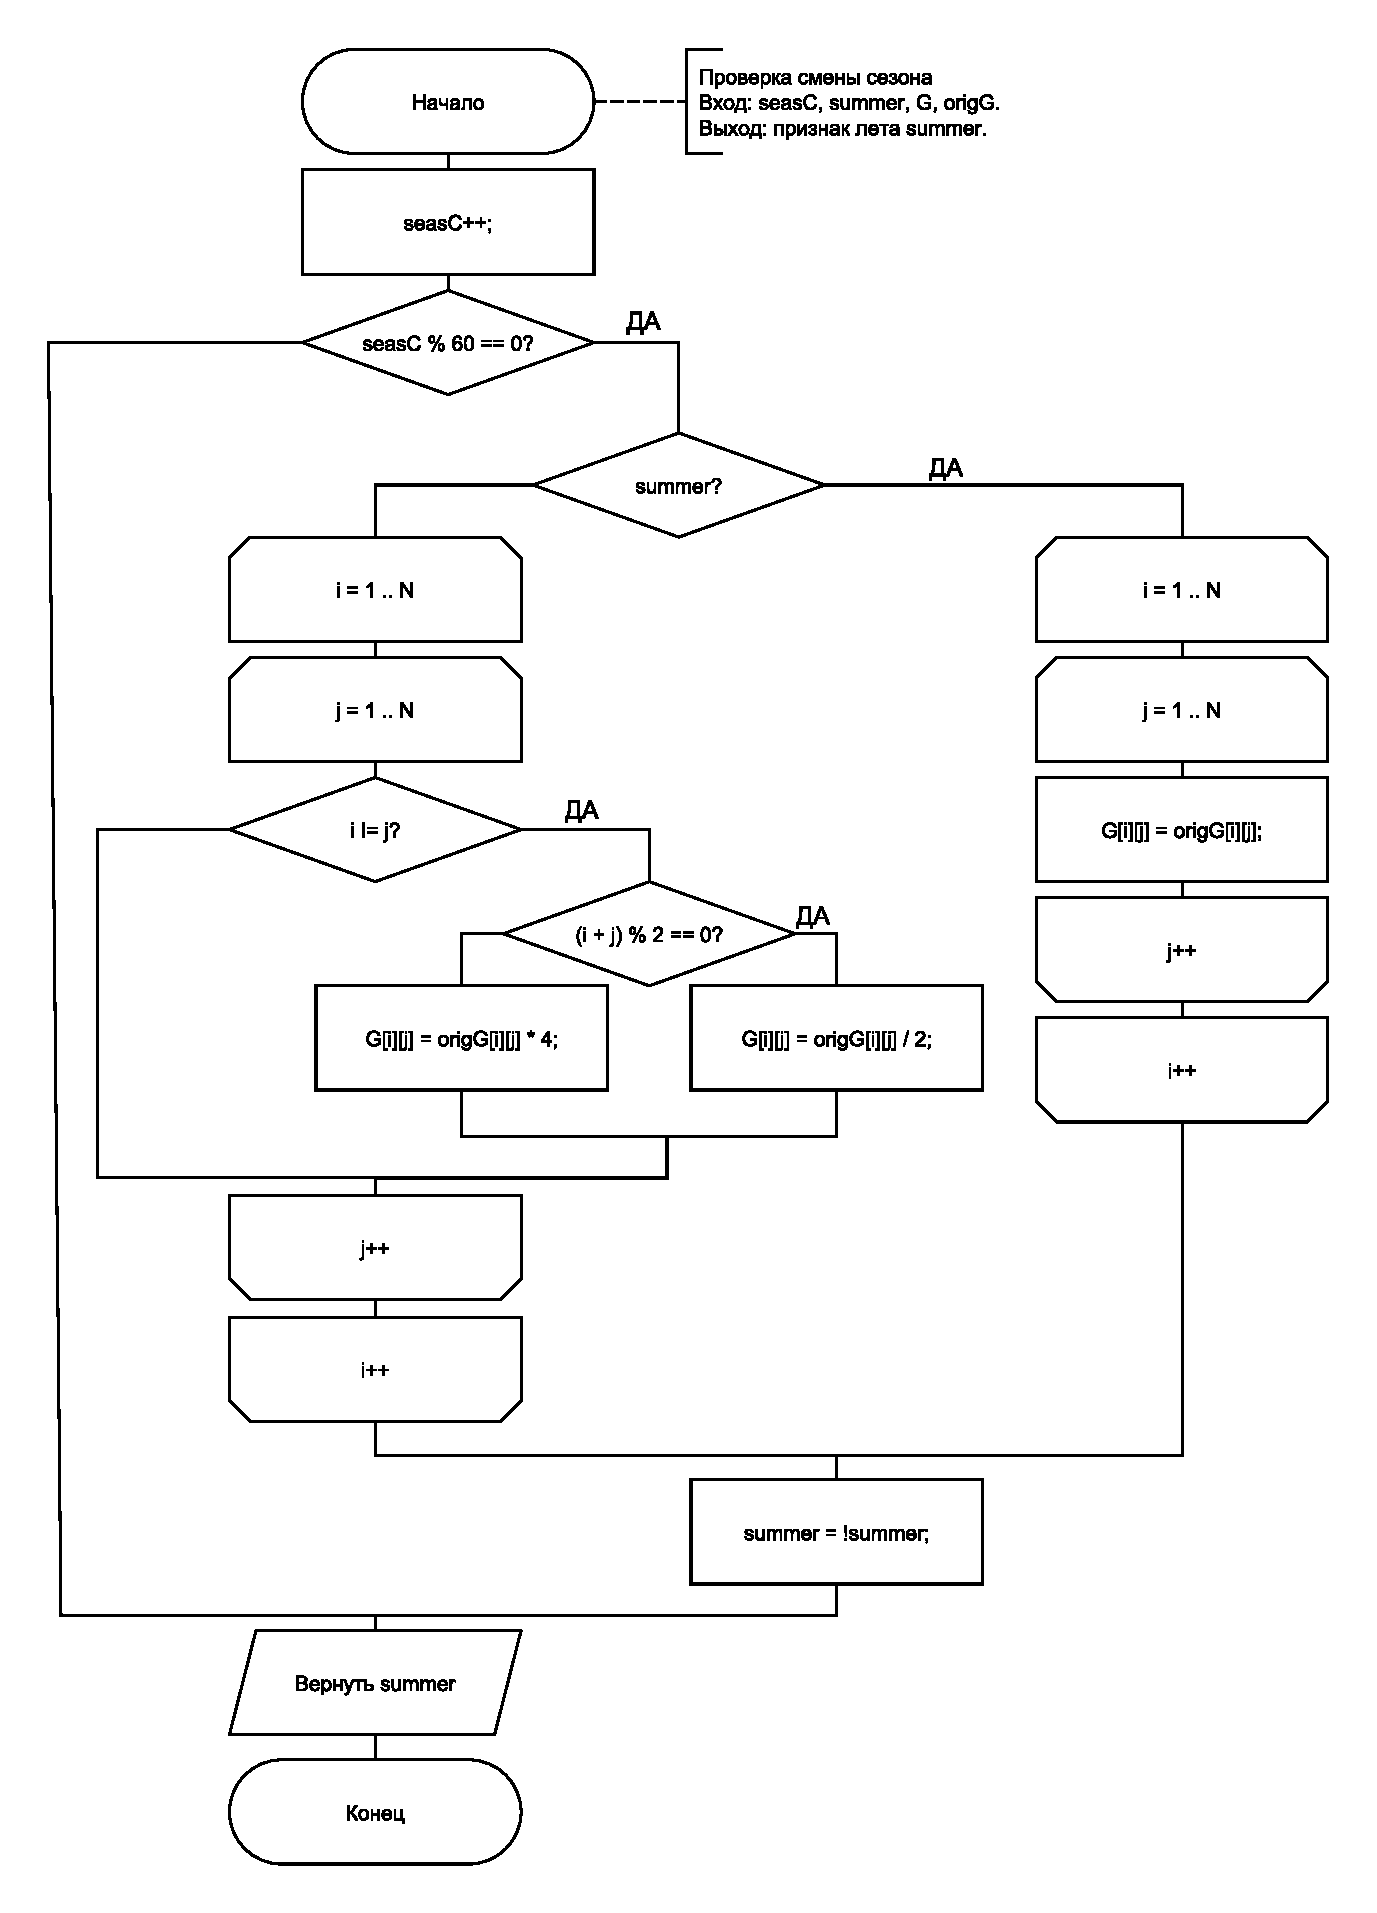
\includegraphics[scale=0.75]{img/season.eps}
	\caption{Схема смены сезона}
	\label{fig:season}
\end{figure}

\clearpage

\section{Модель вычислений}
Для последующего вычисления трудоемкости была введена модель вычислений:
\begin{enumerate}
	\item операции из списка (~\ref{for:opers}) имеют трудоемкость 1;
	\begin{equation}
		\label{for:opers}
		+, -, ==, !=, <, >, <=, >=, [], ++, {-}-, \&\&, ||;
	\end{equation}
    \item операции из списка (~\ref{for:opers}) имеют трудоемкость 2;
	\begin{equation}
		\label{for:opers}
		*, /, \%, pow,
	\end{equation}
    где $pow$ - операция возведения в степень.
	\item трудоемкость условного оператора \code{if условие then A else B} рассчитывается как (~\ref{for:if});
	\begin{equation}
		\label{for:if}
		f_{if} = f_{\text{условия}} +
		\begin{cases}
			f_A, & \text{если условие выполняется,}\\
			f_B, & \text{иначе.}
		\end{cases}
	\end{equation}
	\item трудоемкость цикла рассчитывается как (~\ref{for:for});
	\begin{equation}
		\label{for:for}
		f_{for} = f_{\text{инициализации}} + f_{\text{сравнения}} + N(f_{\text{тела}} + f_{\text{инкремента}} + f_{\text{сравнения}})
	\end{equation}
	\item трудоемкость вызова функции/возврата результата равна 0.
\end{enumerate}


\section{Трудоемкость алгоритмов}
В следующих частях будут рассчитаны трудоемкости представленных ранее алгоритма полного перебора и муравьиного алгоритма.
Трудоемкость начальной инициализации переменных $minCost$ и $bestRoute$, поскольку данное действие есть во всех алгоритмах и не является самым трудоемким.

Введем обозначения:
\begin{itemize}
	\item[---] $N$ --- кол-во строк и столбцов матрицы стоимостей;
    \item[---] $t_{max}$ --- кол-во итераций;
    \item[---] $K$ --- кол-во муравьев;
    \item[---] $E$ --- кол-во элитных муравьев.
\end{itemize}

\subsection{Алгоритм полного перебора}

Трудоемкость алгоритма полного перебора для решения задачи коммивояжера состоит из:

\begin{itemize}
	\item[---] генерации всех перестановок $N$ городов, трудоемкость которой:
    \begin{equation}
        f = N! \cdot N;
    \end{equation}
	\item[---] обработки каждой перестановки, трудоемкость которой:
    \begin{equation}
        f = f_{\textup{ПВМ}}+f_{\textup{ВСМ}}+f_{\textup{обновления}};
    \end{equation}
	\item[---] проверка валидности маршрута (ПВМ) требует $N-1$ сравнения, а значит трудоемкость этого этапа равняется:
    \begin{equation}
        f_{\textup{ПВМ}} = N - 1;
    \end{equation}
    \item[---] вычисление стоимости маршрута (ВСМ) подразумевает суммирование стоимостей переходов между городами, трудоемкость считается как:
    \begin{equation}
        f_{\textup{ВСМ}} = 3 \cdot (N-1);
    \end{equation}
    \item[---] при обновлении значений маршрута и длины проводятся 2 сравнения и 2 присваивания, трудоемкость которых равна:
    \begin{equation}
        f_{\textup{обновления}} = 4;
    \end{equation}
\end{itemize}

В итоге трудоемкость алгоритма полного перебора равна:
\begin{equation}
	\label{for:classic}
	f_{bruteforce} = N! \cdot N + N - 1 + 3 \cdot (N-1) + 4 = N! \cdot N + 4N
\end{equation}

\subsection{Муравьиный алгоритм}

Трудоемкость муравьиного алгоритма состоит из:
\begin{itemize}
    \item[---] инициализации параметров, трудоемкость которой пренебрежимо мала по сравнению с другими этапами:
    \begin{equation}
        f = 1;
    \end{equation}
	\item[---] инициализация матрицы феромонов pher:
	\begin{equation}
		f_{init} = N^2;
	\end{equation}
	\item[---] основного цикла по итерациям:
	\begin{equation}
		f_{tmax} = 2 + t_{max} \cdot (f_{t});
	\end{equation}
	\item[---] цикла по муравьям:
	\begin{equation}
		f_{t} = 2 + K \cdot (f_{k});
	\end{equation}
    \item[---] начальной инициализации параметров муравья (tour, visited, curCity):
	\begin{equation}
		f_{initK} = 2 + N + 3=N+5;
	\end{equation}
    \item[---] построения маршрута, количество шагов которого равно $N$, а для каждого непосещенного города i вычисляется вероятность перехода, значит общая трудоемкость данного этапа равна:
	\begin{equation}
		f_{buildR} = 3 + N + 2 + N \cdot (2 + N + 2 + N \cdot (2 + 7 + 14 + 2) + 4) = 5 + 9N + 26N^2;
	\end{equation}
    \item[---] выбора нового города:
	\begin{equation}
		f_{chooseR} = 2 + N \cdot (N + N) = 2+2N^2;
	\end{equation}
    \item[---] вычисления длины маршрута:
	\begin{equation}
		f_{len} = 2 + (N - 1) = N + 1;
	\end{equation}
    Значит трудоемкость цикла по муравьям равна:
    \begin{equation}
		f_{t} = 2 + K \cdot (N+5+5 + 9N + 26N^2+2+2N^2+N + 1)=2+K(13+11N+28N^2);
	\end{equation}
    \item[---] обновления феромонов:
	\begin{equation}
		f_{pher} \approx N^2;
	\end{equation}
    \item[---] нанесение феромонов муравьями и элитными муравьями:
	\begin{equation}
		f_{addpher} \approx K\cdot N + E\cdot N;
	\end{equation}
    \item[---] смены сезона:
	\begin{equation}
		f_{season} = 5 + 2 + N\cdot(2 + N\cdot (5+2 + 5)) = 7+2N+12N^2;
	\end{equation}

Итого, результирующая трудоемкость муравьиного алгоритма равна (~\ref{for:final})
\begin{equation}
	\label{for:final}
	f_{final} = 1+f_{init} + 2 + t_{max}\cdot(f_{t} + f_{pher} + f_{addpher} + f_{season});
\end{equation}
\begin{equation}
	f_{final} \approx 28t_{max}\cdot N^2K \approx 28N^4.
\end{equation}

\vspace{5mm}

\textbf{ВЫВОД}

 В данном разделе были представлены схемы алгоритмов для решения задачи коммивояжера, а также приведены трудоемкости каждого из алгоритмов.

\clearpage